\documentclass[tikz,border=5]{standalone}

\usetikzlibrary{decorations}

\pgfkeys{/pgf/decoration/.cd,
  stipple density/.store in=\pgfstippledensity,
  stipple density=.1,
  stipple scaling function/.store in=\pgfstipplescalingfunction,
  stipple scaling function=sin(\pgfstipplex*180)*0.875+0.125,
  stipple radius/.store in=\pgfstippleradius,
  stipple radius=0.25pt
}

\pgfdeclaredecoration{stipple}{draw}{
\state{draw}[width=\pgfdecorationsegmentlength]{%
  \pgfmathparse{\pgfdecoratedcompleteddistance/\pgfdecoratedpathlength}%
  \let\pgfstipplex=\pgfmathresult%
  \pgfmathparse{int(\pgfstippledensity*100)}%
  \let\pgfstipplen=\pgfmathresult%
  \pgfmathloop%
  \ifnum\pgfmathcounter<\pgfmathresult\relax%
    \pgfpathcircle{%
      \pgfpoint{(rnd)*\pgfdecorationsegmentlength}%
        {(\pgfstipplescalingfunction)*(rnd^4)*\pgfdecorationsegmentamplitude+\pgfstippleradius}}%
    {\pgfstippleradius}%
  \repeatpgfmathloop%
}
}

\tikzset{stipple/.style={
  decoration={stipple, segment length=2pt, #1},
  decorate,
  fill
}}
\begin{document}
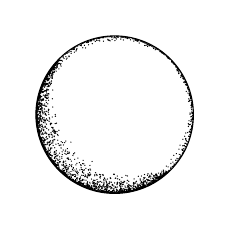
\begin{tikzpicture}
	\draw [postaction={stipple={amplitude=0.125cm}}]
	(0,0) [rotate=45]  circle [radius=1];
	\path [postaction={stipple={amplitude=0.25cm, stipple density=.35}},
		postaction={stipple={amplitude=0.35cm, stipple density=.15}}]
	(135:1) arc (135:315:1);
\end{tikzpicture}

\end{document}

